\documentclass[11pt,a4paper]{article}
\usepackage[spanish,es-nodecimaldot]{babel}	% Utilizar español
\usepackage[utf8]{inputenc}					% Caracteres UTF-8
\usepackage{graphicx}						% Imagenes

\PassOptionsToPackage{hyphens}{url}
\usepackage[hidelinks]{hyperref}			% Poner enlaces sin marcarlos en rojo

\usepackage{fancyhdr}						% Modificar encabezados y pies de pagina
\usepackage{float}							% Insertar figuras
\usepackage[textwidth=390pt]{geometry}		% Anchura de la pagina
\usepackage[nottoc]{tocbibind}				% Referencias (no incluir num pagina indice en Indice)
\usepackage{enumitem}						% Permitir enumerate con distintos simbolos
\usepackage[T1]{fontenc}					% Usar textsc en sections
\usepackage{amsmath}						% Símbolos matemáticos
\usepackage{listings}
\usepackage{algorithm}
\usepackage{amssymb}

% no accents in math operators
\unaccentedoperators

\usepackage{color}
 
\definecolor{codegreen}{rgb}{0,0.6,0}
\definecolor{codegray}{rgb}{0.5,0.5,0.5}
\definecolor{codepurple}{rgb}{0.58,0,0.82}
\definecolor{backcolour}{rgb}{0.95,0.95,0.92}
 
\lstdefinestyle{mystyle}{
    backgroundcolor=\color{backcolour},   
    commentstyle=\color{codegreen},
    keywordstyle=\color{magenta},
    numberstyle=\tiny\color{codegray},
    stringstyle=\color{codepurple},
    basicstyle=\footnotesize,
    breakatwhitespace=false,         
    breaklines=true,                 
    captionpos=b,                    
    keepspaces=true,                 
    numbers=left,                    
    numbersep=5pt,                  
    showspaces=false,                
    showstringspaces=false,
    showtabs=false,                  
    tabsize=2
}
 
\lstset{style=mystyle, language=Python}

% Comando para poner el nombre de la asignatura
\newcommand{\asignatura}{Aprendizaje Automático}
\newcommand{\autor}{Vladislav Nikolov Vasilev}

% Configuracion de encabezados y pies de pagina
\pagestyle{fancy}
\lhead{Vladislav Nikolov, José María Sánchez}
\rhead{\asignatura{}}
\lfoot{Grado en Ingeniería Informática}
\cfoot{}
\rfoot{\thepage}
\renewcommand{\headrulewidth}{0.4pt}		% Linea cabeza de pagina
\renewcommand{\footrulewidth}{0.4pt}		% Linea pie de pagina

\begin{document}
\pagenumbering{gobble}

% Pagina de titulo
\begin{titlepage}

\begin{minipage}{\textwidth}

\centering

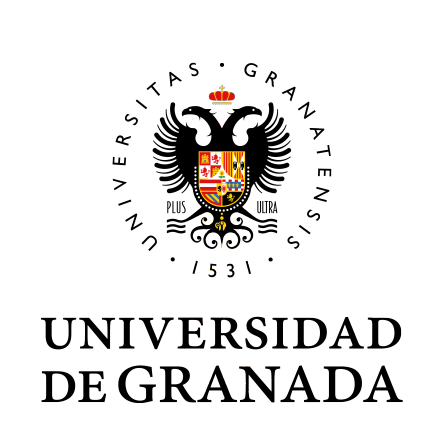
\includegraphics[scale=0.5]{img/ugr.png}\\

\textsc{\Large \asignatura{}\\[0.2cm]}
\textsc{GRADO EN INGENIERÍA INFORMÁTICA}\\[1cm]

\noindent\rule[-1ex]{\textwidth}{1pt}\\[1.5ex]
\textsc{{\Huge PROYECTO FINAL\\[0.5ex]}}
\noindent\rule[-1ex]{\textwidth}{2pt}\\[3.5ex]

\end{minipage}

\vspace{1cm}

\begin{minipage}{\textwidth}

\centering

\textbf{Autores}\\ {\autor{}}\\{José María Sánchez Guerrero}\\[2ex]
\textbf{Rama}\\ {Computación y Sistemas Inteligentes}\\[2ex]
\vspace{0.3cm}


\includegraphics[scale=0.3]{img/etsiit.jpeg}

\vspace{0.7cm}
\textsc{Escuela Técnica Superior de Ingenierías Informática y de Telecomunicación}\\
\vspace{1cm}
\textsc{Curso 2018-2019}
\end{minipage}
\end{titlepage}

\pagenumbering{arabic}
\tableofcontents
\thispagestyle{empty}				% No usar estilo en la pagina de indice


\newpage

\setlength{\parskip}{1em}

\section{\textsc{Descripción del problema}}

El conjunto de datos con el que vamos a trabajar es el \textbf{\textit{Image Segmentation Data Set}}, creado por el Vision Group de
la Universidad de Massachusetts. Este conjunto de datos contiene una serie de características de casos extraídos al azar
de una base de datos con 7 tipos de imágenes tomadas al aire libre. Éstas imágenes fueron segmentadas manualmente para
crear una clasificación para cada píxel. Cada instancia es una región de $3 \times 3$.

Originalmente, nuestro conjunto de datos estaba ya dividido en training y test. Sin embargo, disponemos solo de 210 datos
de entrenamiento y 2100 de test. Como la cantidad de datos que tenemos para entrenamiento es muy inferior a la de test, y
no existe un motivo justificado por el que las particiones se hayan hecho de esta forma, hemos decidido juntar todos los
datos y crear nuestras propias particiones de entrenamiento y test. Esta división se comentará con más detalles en
secciones posteriores, cuando hablemos de las transformaciones y preprocesado que hemos realizado sobre los datos de los
que disponemos. 

Según la información proporcionada por la descripción del conjunto de datos, la cuál puede ser encontrada en el
repositorio UCI \cite{bib:uci-repo}, existen \textbf{7 clases} distintas, y hay 30 muestras de cada clase en el conjunto de
entrenamiento y 300 en el conjunto de test. Con lo cuál, tenemos que en total hay 330 muestras de cada clase si miramos
los dos conjuntos de datos de forma conjunta. En total disponemos de 2310 muestras, cada una de las cuáles tiene \textbf{19
atributos} que toman valores reales. En la representación original de los datos, tenemos que la primera columna se
corresponde con la clase de la muestra, y las 19 columnas restantes se corresponden con los atributos. 

De esta pequeña descripción podemos concluir que cada clase está idénticamente representada en los datos de los que
disponemos, y que no existe una clase que esté representada en mayor o menor medida que el resto de ellas. 

Con todo esto dicho, vamos a proceder a analizar cada una de las 19 características mencionadas anteriormente, para ver
que representa cada una de ellas:

\begin{enumerate}
	\item \textit{Region-centroid-col}: la columna del píxel central de la región.
	\item \textit{Region-centroid-row}: la fila del píxel central de la región. 
	\item \textit{Region-pixel-count}: el número de píxeles en una región. Su valor siempre es 9. 
	\item \textit{Short-line-density-5}: resultados de un algoritmo de extracción de rectas que cuenta cuántas líneas de longitud 5
	(con cualquier orientación) con bajo contraste, menor o igual a 5, cruzan la región. 
	\item \textit{Short-line-density-2}: igual que \textit{Short-line-density-5} pero cuenta con líneas de alto contraste,
	mayor que 5. 
	\item \label{it:vegde} \textit{Vegde-mean}: mide el contraste de píxeles horizontalmente adyacentes en la región. Hay 6 valores,
	pero se da dan la media y la desviación típica. Este atributo se utiliza como un detector de borde vertical. 
	\item \textit{Vegde-sd:} Desviación típica del contraste de píxeles horizontalmente adyacentes en la región (ver \ref{it:vegde}).
	\item \label{it:hedge} \textit{Hedge-mean}: mide el contraste de los píxeles verticalmente adyacentes.
	Utilizado para la detección de líneas horizontales. Este atributo es el valor medio.
	\item \textit{Hedge-sd}: Desviación típica del contraste de los píxeles verticalmente adyacentes (ver \ref{it:hedge}). 
	\item \textit{Intensity-mean}: el promedio sobre la región de (R + G + B) / 3.
	\item \textit{Rawred-mean}: Promedio sobre la región del valor R. 
	\item \textit{Rawblue-mean}: Promedio sobre la región del valor B. 
	\item \textit{Rawgreen-mean}: Promedio sobre la región del valor G. 
	\item \textit{Exred-mean}: Mide el exceso de rojo: (2R - (G + B)).
	\item \textit{Exblue-mean}: Mide el exceso de azul: (2B - (G + R)).
	\item \textit{Exgreen-mean}: Mide el exceso de verde: (2G - (R + B)).
	\item \label{it:value} \textit{Value-mean}: Transformación 3D no lineal de RGB.
	\item \textit{Saturatoin-mean}: (ver \ref{it:value}).
	\item \textit{Hue-mean}: (ver \ref{it:value}).
\end{enumerate}

Como estamos en un problema de clasificación, cada entrada produce una salida que es una etiqueta. La etiqueta puede hacer
referencia a una de las 7 clases que tiene el problema, las cuáles son: \textit{brickface}, \textit{sky},
\textit{foliage}, \textit{cement}, \textit{window}, \textit{path} y \textit{grass}. Para facilitar la representación de
las clases, vamos a transformar posteriormente cada valor de las etiquetas a un valor numérico. Esto se verá con más
detalle en secciones posteriores, cuando hablemos del preprocesado de los datos de entrada.

\newpage

\section{\textsc{Enfoque elegido para el análisis}}

El análisis y la elección de los modelos para nuestro problema va a tener varias fases, las cuales vamos a detallar a continuación:
\begin{itemize}[label=\textbullet]
\item Lo primero será el \textbf{preprocesado y análisis de los datos}, donde empezaremos leyendo los datos de los ficheros
proporcionados y los manipularemos para obtener un conjunto de datos con el que trabajaremos más cómodamente. Posteriormente se realizará
un estudio del conjunto de datos con la finalidad de conocer mejor el problema y cada uno de sus atributos y clases.
\item Después elegiremos las \textbf{métricas a utilizar}, donde seleccionaremos una serie de valores que nos permitan comparar los modelos.
Con una buena métrica podremos ver cómo de bueno es el rendimiento que nos ofrecen.
\item A continuación, \textbf{seleccionaremos los modelos a evaluar } y comentaremos brevemente cuáles son las \textbf{funciones de pérdida}
que utiliza cada modelo, además de comentar muy brevemente la aplicación de regularización a cada modelo.
\item Tras seleccionarlos tocará \textbf{evaluar y comparar los distintos modelos}, donde describiremos con más detalle la metodología
de evaluación seguida, probaremos los distintos modelos, analizaremos los resultados obtenidos y, a partir de ellos, compararemos el
rendimiento ofrecido por cada uno de ellos.
\item Una vez hayamos analizado los modelos, tendremos que \textbf{elegir y ajustar los mejores modelos}, donde utilizaremos los resultados
anteriores para seleccionar los que hayan funcionado mejor y luego ajustaremos sus hiperparámetros para intentar mejorarlos aun más.
\item Por último, vamos a \textbf{evaluar el mejor modelo}, es decir, una vez ajustados los mejores y decido cuál es el que nos va a resultar
más útil en nuestro problema, veremos como se enfrenta al conjunto de test. Analizaremos los resultados y concluiremos si hemos tomado una
buena decisión al elegir ese modelo.
\end{itemize}

\newpage

\section{\textsc{Preprocesado de los datos de entrada}}

En esta sección vamos a comentar el preprocesado que hemos hecho a los datos de entrada. Es decir, vamos a ver cómo y por qué juntamos
los dos conjuntos de datos y luego los separamos (tal y como dijimos en la sección anterior) y vamos a ver que modificaciones hacemos
sobre éstos para que nos sea más fácil trabajar posteriormente con ellos y para adaptarlos mejor al problema que queremos resolver.

Vamos a comenzar leyendo los datos y almacenándolos en estructuras de datos que nos permitan el fácil acceso a éstos. Posteriormente,
tal y como dijimos anteriormente, vamos a juntar los dos conjuntos en uno solo. Esto se puede ver a continuación:

\begin{lstlisting}
# Leer los datos de training y test
df1 = read_data_values('datos/segmentation.data')
df2 = read_data_values('datos/segmentation.test')

# Juntar los dos conjuntos en uno solo
df = pd.concat([df1,df2])
\end{lstlisting}

Nuestro objetivo al hacer esto es disponer de todos los datos de \textbf{forma conjunta} para luego poder crear nuestras propias particiones de
entrenamiento y de test, debido a que, como hemos dicho anteriormente, la cantidad de datos de entrenamiento de la que disponemos es
muy pequeña. Como no existe una justificación para no crear nuestras propias particiones, vamos a crearlas de tal forma que tengamos más
datos de entrenamiento que de test, conservando además la forma en la que cada clase está representada. Con esto, obtendremos un 
mejor modelo, ya que tendremos más datos con los que entrenarlo, y por tanto, va a generalizar mejor.

Sin embargo, antes de realizar las particiones, vamos a transformar las clases originales a valores numéricos, para que el trabajar
con ellas posteriormente sea más sencillo. Vamos a asignar a cada etiqueta un número. Como tenemos 7 clases, asignaremos un número
en el rango $[0, 6]$ a cada una de ellas, de forma que no se repita ningún número para ninguna etiqueta. Esta asignación se puede ver a
continuación:

\begin{lstlisting}
# Valor numerico asignado a cada etiqueta
labels_to_values = { 'BRICKFACE' : 0, 'SKY' : 1, 'FOLIAGE' : 2,
                     'CEMENT': 3, 'WINDOW' : 4, 'PATH' : 5,
                     'GRASS' : 6 }
\end{lstlisting}

Ahora ya solo nos quedaría aplicar el \textit{mapping}. Como todavía no hemos separado las etiquetas de los datos y sabiendo que, gracias
a la información proporcionada por el repositorio, la etiqueta se encuentra en la primera columna, la sustitución se puede hacer de forma
sencilla de la siguiente manera:

\begin{lstlisting}
# Sustituir etiquetas de salida por valores numericos discretos
df[0] = df[0].map(labels_to_values)
\end{lstlisting}

Con esto ya hecho, ya podemos dividir los datos en los valores de entrada $\mathcal{X}$ y las etiquetas $y$ y posteriormente dividir
éstos en los conjuntos de entrenamiento y de test. Queremos que el \textbf{80\%} de los datos de los que disponemos esté en el conjunto de
\textbf{entrenamiento} y que el \textbf{20\%} restante esté en el de \textbf{test}. Además, tal y como se mencionó anteriormente, queremos que las clases estén
igualmente representadas en los dos conjuntos en función de la cantidad de muestras que hay en total de cada clase. También es importante
mezclar los datos, con tal de que la elección de qué muestra va a cada conjunto no sea decidida por el orden de las muestras, si
no que se haga de forma aleatoria.

Se ha escogido esta repartición de los datos ya que nos permite tener un número suficientemente grande de muestras para entrenar nuestro
modelo y una cantidad aceptable de datos para ver como se desempeña con datos nunca vistos antes. La desventaja de hacer \textit{hold-out}
(que es lo que estamos haciendo aquí) es que perdemos datos para entrenar nuestro modelo, datos con los que, muy posiblemente, pudiésemos
obtener unos mejores resultados. Sin embargo, siguiendo este enfoque, tendremos al menos una forma de ver cómo de bien funciona nuestro
modelo con nuevos datos con los que nunca antes había interaccionado.

Vamos a ver ahora como se realizaría esta partición de los datos:

\begin{lstlisting}
# Obtener valores X, Y
X, y = divide_data_labels(df)

# Dividir los datos en training y test
# Conservar proporcionalidad de clase mezclando los datos
print('Splitting data in training and test sets...')
X_train, X_test, y_train, y_test = train_test_split(
        X, y, test_size=0.2, random_state=1, shuffle=True, stratify=y)
\end{lstlisting}

Y con todo esto visto, pasemos ahora a la parte de análisis de los datos, la cuál nos va a permitir obtener más información acerca de
los datos de los que disponemos.

\newpage

\section{\textsc{Análisis de los datos}}

En esta sección vamos a realizar un estudio de los datos para ver qué información nos pueden ofrecer sobre el problema. Lo primero que
vamos a hacer es observar algunas muestras del conjunto de entrenamiento para hacernos una idea de cómo es y qué valores pueden tomar
algunos de los atributos. Esto se puede ver a continuación:

\begin{figure}[H]
    \centering
    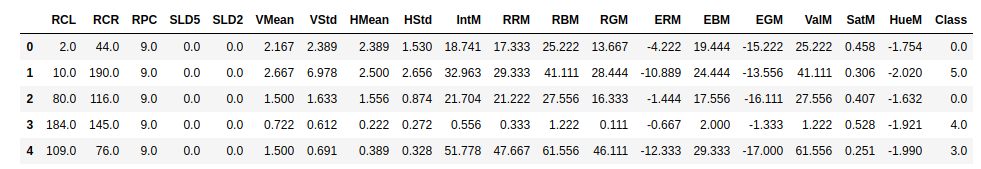
\includegraphics[scale=0.4]{img/train_df_head.png}
    \caption{Ejemplo del conjunto de datos de entrenamiento.}
    \label{fig:train-df}
\end{figure}

Una vez hecho esto, vamos a comprobar, para asegurarnos, cuáles son los tamaños de los conjuntos de entrenamiento y de test, y ver
si falta algún valor en estos conjuntos (a pesar de que en el repositorio se indicaba que no falta ninguno, nunca viene mal asegurarse).
Veamos a continuación qué información podemos extraer de aquí:

\begin{lstlisting}
# Determinar numero de muestras por conjunto
print('Training data size: ', train_df.shape[0])
print('Test data size: ', test_df.shape[0])

# Determinar si faltan valores para los dos conjunts
print('Missing values in train? ', train_df.isnull().values.any())
print('Missing values in test? ', test_df.isnull().values.any())
\end{lstlisting}

\begin{figure}[H]
    \centering
    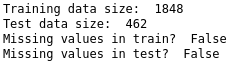
\includegraphics[scale=0.6]{img/df_info.png}
    \caption{Información sobre los tamaños de los conjuntos y la cantidad de valores que faltan.}
    \label{fig:train-test-stat}
\end{figure}

Podemos ver que el conjunto de entrenamiento tiene ahora 1848 muestras, mientras que el de test tiene 462. Estos nuevos tamaños son
resultado de la partición que hemos hecho anteriormente, y podemos ver claramente que el 20\% de los datos totales están en el
conjunto de test, tal y como habíamos especificado. Estos tamaños son más adecuados para entrenar los modelos, ya que al tener más
datos de entrenamiento, y si esta cantidad es lo suficientemente grande, los modelos podrán ser capaces de generalizar mejor. Como
al principio solo teníamos 200 datos de entrenamiento, la capacidad de generalizar de los modelos estaba más limitada. Aparte, tenemos
una cantidad de datos suficiente para poder probar luego nuestro modelo, para ver como se comporta con nuevos datos.

Pasemos ahora a estudiar un aspecto bastante importante de los datos que es la correlación de éstos. Nos interesa ver si existe
\textbf{correlación lineal} entre los datos de entrada y los de salida, para ver si sería necesario eliminar algún atributo. Además, también es
interesante ver si existe alguna correlación entre los atributos que tenemos como entrada. A continuación, se muestra la \textbf{matriz de
correlación} de los datos de entrenamiento, y sobre ella vamos a ir comentando los resultados:

\begin{figure}[H]
    \centering
    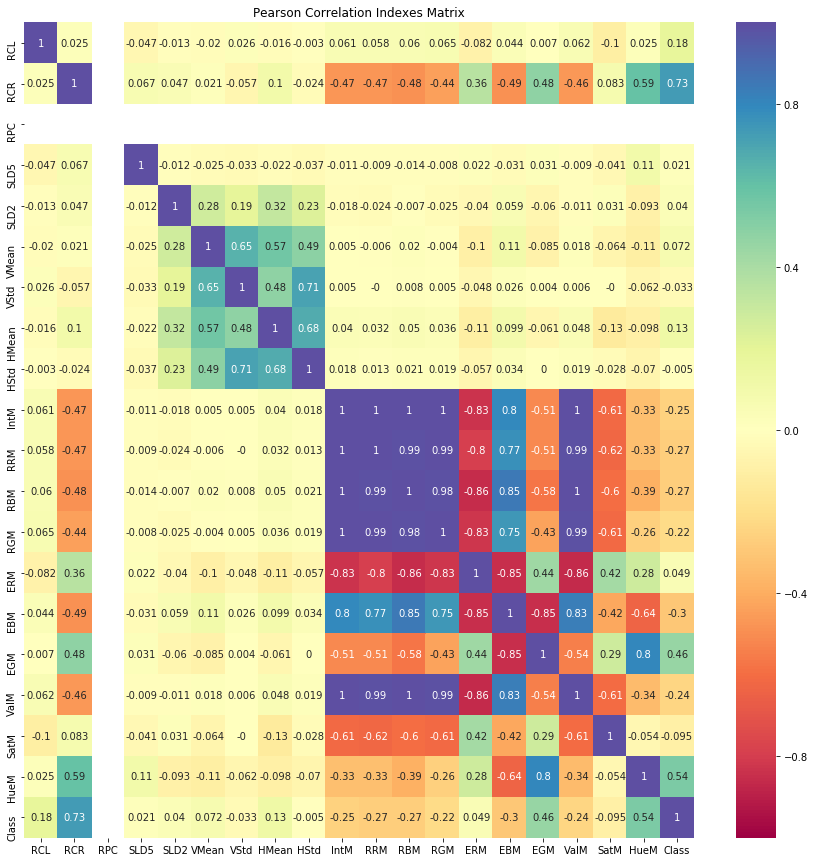
\includegraphics[scale=0.4]{img/correlation.png}
    \caption{Matriz con los coeficientes de correlación de Pearson.}
    \label{fig:pearson}
\end{figure}

De la figura anterior, podemos sacar algunas conclusiones:

\begin{itemize}[label=\textbullet]
    \item Tal y como nos indicaba la información del repositorio, existe un atributo que es constante, y que por tanto, no aporta
    ninguna información. Este atributo es el \textit{Region-pixel-count}, y se puede ver que en la figura no aparece ninguna
    información sobre éste. Por tanto, al ser un atributo ``inútil'', \textbf{va a ser eliminado}.
    \item Según lo que nos indica el gráfico, existen algunas variables que parecen tener una correlación mayor con la salida que
    otras. Por ejemplo, el \textit{Region-centroid-row} tiene una correlación de 0.73, un valor bastante alto. Sin embargo, al estar
    en un problema de clasificación, esta correlación no indica mucha información, ya que la salida es un valor discreto en vez de
    uno continuo, y por tanto, que la variable crezca o decrezca no parece indicar mucho en cómo va a afectar a la salida, ya que ésta
    es un valor discreto y no uno continuo.
    \item Existen una serie de variables de entrada que están bastante correlacionadas entre sí, ya que sus coeficientes de correlación de
    Pearson son 1, lo cuál significa que existe una correlación lineal entre ellas y que siempre que alguna de ellas crezca, la otra también
    lo hará. Esto nos podría indicar que podríamos eliminar algunos de estos atributos, ya que en un principio parecen aportar información
    redundante. Sin embargo, \textbf{no vamos a eliminar ninguna de las variables de entrada correlacionadas}, debido a que si decidimos
    eliminarlas a mano solo por tener una correlación lineal podríamos estar cometiendo un error, ya que nada nos asegura que esas variables
    no aportan información útil. Además, estaríamos tomando decisiones que podrían afectar posteriormente al modelo, y por tanto, sería
    mejor dejar que los modelos como tal decidan si esas variables son importantes o no en vez de hacerlo nosotros.
\end{itemize}

Con esto dicho, ya que hemos visto que existe una variable que no nos aporta ninguna información por el hecho de que es \textbf{constante}, vamos
a eliminarla tanto del conjunto de entrenamiento como el de test. Esto lo vamos a hacer a continuación mediante el siguiente código:

\begin{lstlisting}
# Crear lista de variables a eliminar
rm_list = [2]

# Eliminar variables de training y test
X_train = np.delete(X_train, rm_list, axis=1)
X_test = np.delete(X_test, rm_list, axis=1)
\end{lstlisting}

Habiendo eliminado esta variable, nos quedamos con 18 variables que vamos a utilizar en nuestro problema. Cada modelo ponderará a estas
variables de una forma u otra, dándoles diferente importancia.

Una vez concluido este pequeño análisis, vamos a pasar a comentar qué métricas vamos a utilizar para evaluar los modelos, antes de ver
exactamente cuáles de ellos utilizaremos.

\newpage

\section{\textsc{Elección de las métricas a utilizar}}

Está claro que, para comparar los distintos modelos y elegir a los mejores de entre ellos, necesitamos alguna \textbf{métrica} que nos permita
ver cómo de buenos son sus rendimientos. Como estamos en un problema de clasificación, parece que la \textbf{\textit{accuracy}} es una buena
elección, ya que es una métrica que indica cuántos elementos ha predicho el modelo correctamente sobre el número total de elementos. Además
de eso, la interpretación de esta métrica es muy sencilla e intuitiva, lo cuál no hace más que acentuar su idoneidad en este caso. Y,
aparte, es una muy buena métrica cuando el número de muestras que hay en cada clase está equilibrado, como es este caso, ya que los
resultados obtenidos son más representativos. En caso de no estar equilibradas, por ejemplo, si el 90\% de las muestras fuesen de una clase
y el 10\% fuese de otra, el clasificador podría tener una \textit{accuracy} de 90\%, pero podría estar clasificando correctamente solo
elementos de la clase predominante.

Con el modelo ya elegido, nos interesaría conocer algo más de información sobre su rendimiento, aparte de la \textit{accuracy}. Sería
interesante, por ejemplo, saber cómo clasifica con más detalle, viendo por ejemplo cuántos y qué elementos de cada clase clasifica
correctamente y en cuántos y cuáles de ellos se equivoca y en qué clase los clasifica. Esto se puede obtener mediante la
\textbf{matriz de confusión}. Esta matriz, además, nos permite obtener dos métricas más que tienen cierto interés.

Una de ellas es el \textbf{\textit{recall} o sensibilidad}, métrica que nos indica la proporción de elementos que pertenecen a una clase han sido
clasificados de forma correcta respecto al total de elementos que hay verdaderamente en esa clase. Esta métrica nos permite medir la
capacidad que tiene el clasificador de \textit{encontrar todas las muestras positivas}\cite{bib:recall}. Es decir, si tenemos que $TP$
(\textit{True Positives} o verdaderos positivos, a lo que se refiere con \textit{muestra positiva}) son los elementos de una clase
clasificados correctamente, y $FN$ (\textit{False Negatives} o falsos negativos) los elementos de una clase que han sido clasificados como
elementos de otra/s clases, tenemos que:

\[ 
\text{Recall} = \frac{TP}{TP + FN}
\]

La otra métrica es la \textbf{\textit{precision} o precisión}, la cuál nos indica qué proporción de elementos predichos de una clase se corresponden
a la clase real respecto a la cantidad total de elementos predichos de esa misma clase. Esta métrica nos permite medir la capacidad que tiene
el clasificador de \textit{no clasificar una muestra negativa como positiva}\cite{bib:precision}. Es decir, si tenemos que $TP$ son los
elementos de una clase clasificados correctamente, y que los $FP$ (\textit{False Positives} o falsos positivos, a lo que se refiere con
\textit{muestra negativa}) son los elementos que se han predicho que pertenecen a una determinada clase pero que en realidad pertenecen a
otra pertenecen a otra, tenemos que:

\[ 
\text{Precision} = \frac{TP}{TP + FP}
\]

De estas dos métricas, nos interesa obtener valores medios, ya que estamos en un problema de clasificación en el que hay múltiples clases.
Con lo cuál, nos interesa saber, de media, qué valores de \textit{recall} y \textit{precision} obtiene nuestro clasificador.

\section{\textsc{Elección de los modelos a evaluar}}

Una vez que hemos hablado de las métricas que vamos a utilizar para evaluar los distintos modelos, es hora de pasar a comentar la parte más
importante de todas, sin la cuál no tendría sentido nada de lo que estamos haciendo: los modelos. Hablaremos brevemente de qué modelos hemos
elegido y el por qué de cada uno de ellos.

\subsection{Regresión Logística Multinomial}

El primer modelo que hemos elegido es la \textbf{Regresión Logística Multinomial}, el cuál es un modelo lineal y es una generalización de la Regresión
Logística para múltiples clases. Esto último ha sido uno de los motivos principales por los que ha sido escogido, ya que permite trabajar con
múltiples clases, que es justamente lo que tenemos en este problema.

Existen otros muchos modelos que son variantes de la Regresión Logística para múltiples clases, como por ejemplo la Regresión Logística con
\textit{one-vs-rest}, donde se tienen $K$ modelos diferentes, donde $K$ es el número de clases. Cada modelo es un clasificador binario que
mide la probabilidad de que el elemento pertenezca a esa clase y la probabilidad de que el elemento no pertenezca a esa clase. Sin embargo,
en la Regresión Logística Multinomial hay un solo modelo que da $K$ probabilidades, las cuáles indican la probabilidad de que el elemento
pertenezca a cada una de las $K$ clases. Esto otra ventaja, ya que es mucho más intuitivo saber cuáles es la probabilidad real de pertenecer
a cada una de las $K$ clases para un dato de entrada.

La función de pérdida o \textit{loss function} que utiliza este modelo es la \textbf{Multi-class Cross Entropy}, una generalización de la
\textbf{Cross Entropy}, la cuál se utiliza en la Regresión Logística para dos clases. Esta función viene dada por la siguiente expresión:

\begin{equation}
\label{eq:mult-cross-entropy}
E(\mathbf{w_1}, \mathbf{w_2}, \dots, \mathbf{w}_K) = -\sum_{n=1}^N \sum_{k=1}^{K} y_{nk} \ln \Big(\sigma (\mathbf{w}_K^T \mathbf{x}_n)\Big)
\end{equation}

En cuanto a la \textbf{regularización}, como sabemos, nunca viene mal regularizar el modelo que estamos entrenando, ya que evitamos problemas de
\textit{overfitting} o sobreajuste, siempre y cuando el valor de $\lambda$ (hiperparámetro que pondera la regularización) sea el adecuado. 
En este caso, el modelo utilizará regularización de tipo $\ell 2$, debido a que la regularización $\ell 1$ se encargaría de eliminar ciertas
características asignándoles el valor 0, considerándolas como poco importantes. Al tener nosotros un número bastante pequeño de
características, no nos interesa mucho eliminar alguna de ellas, ya que podríamos perder información significativa.

\subsection{Support Vector Machine con \textit{kernel} RBF}

El segundo modelo que queremos evaluar es el \textbf{SVM con \textit{kernel} RBF}, un \textit{kernel} no lineal. Se ha escogido este \textit{kernel}
porque en general, en problemas de clasificación ofrece resultados bastante buenos y es bastante rápido. Hemos escogido este modelo porque,
aparte de encontrar una separación entre las clases, SVM también intenta buscar la separación óptima, dejando un margen suficiente a cada
lado, de forma que ningún punto caiga dentro de ese margen. Por tanto, está buscando también una separación \textbf{óptima} entre las clases.

Como muchas veces esto no es posible o los datos no son linealmente separables, se tienen que tolerar algunas violaciones de margen, dejando
que haya puntos dentro del margen o que no se hayan clasificado bien. Esto viene definido por el hiperparámetro $C$, el cuál indica cuál
es la importancia asociada a esta violación del margen. A menor peso, menos importancia, y por tanto, se consigue una separación más
regularizada y un margen más grande.

Este modelo funciona de forma diferente al SVM con \textit{kernel} lineal, ya que clasifica los datos por similaridad a los de la muestra.
Esta similaridad viene dada por la distancia euclídea. A mayor similaridad, menor la distancia. También está influida por un parámetro
$\gamma$, el cuál indica cuál es la influencia de ese punto. A mayor $\gamma$, menor influencia tendrán los puntos de la muestra, con lo cuál,
solo puntos muy cercanos a ellos podrán clasificarse como cercanos. A menor $\gamma$, más influencia tendrán los puntos de la muestra, y por
tanto, un nuevo punto podrá ser considerado como similar aún situándose bastante lejos del de la muestra. Este parámetro también define
cierto grado la regularización, ya que cuanto mayor sea el valor, mayor tendencia al sobreajuste, mientras que si es demasiado pequeño,
el modelo puede quedarse corto y sufrir de \textit{underfitting}.

La función de pérdida que utiliza este modelo, al igual que las otras variantes de SVM, es el \textbf{Hinge Loss}, el cuál tiene la siguiente
forma:

\begin{equation}
\label{eq:hinge-loss}
E_{SVM}(b, \mathbf{w}) = \frac{1}{N} \sum_{n=1}^N \max(1 - y_n \mathbf{w}^T\mathbf{x}_n + b , 0)
\end{equation}

\noindent la cuál no puede ser minimizada directamente al no ser derivable, si no que debe ser transformada y se debe resolver en el problema
dual. Se ha escogido esta función de pérdida debido a que es la que nos permite maximizar el margen que se deja a cada lado de la separación
entre las clases.

En cuanto a la \textbf{regularización}, hay dos parámetros que influyen que se han comentado anteriormente, que son $\gamma$ y $C$. Por tanto, se
intentará controlar el parámetro $C$ a la hora de evaluar el modelo para hacer que no se obtenga un modelo muy ajustado a los puntos, y por
tanto, con sobreajuste.

\subsection{Random Forest}

El tercer modelo que queremos evaluar es el \textbf{Random Forest}, el cuál representa una mejora sobre los árboles de decisión clásicos y la técnica
de \textit{bagging}. Este modelo permite tener múltiples árboles de decisión los cuáles son entrenados cada uno con una muestra de datos
escogidos mediante \textit{bootsrap} de la original. Además, cada árbol escoge un subconjunto de predictores que va a utilizar para intentar
predecir, con el objetivo de evitar el problema de \textit{bagging} en el cuál la mayoría de árboles estaban correlacionados. Si
existe un predictor muy fuerte, este será utilizado casi siempre en la primera partición que se hace de los datos en cada árbol, haciendo por
tanto que la mayoría de árboles sea parecido.

Se ha escogido este modelo porque es un modelo que ofrece unos resultados muy buenos en general ya que tiene un bajo sesgo y una baja varianza
al tener múltiples árboles, que además no están correlacionados, lo cuál hace que la media de la varianza del modelo sea aún menor.

Como tal, la técnica de Random Forest \textbf{no utiliza una función de pérdida}, ya que no intenta minimizar nada. Sin embargo, sigue algún tipo de
heurística subyacente que permite construir el árbol con los datos de los que se dispone.

En cuanto a la \textbf{regularización} de este modelo, a pesar de que como tal ya ofrece una varianza baja, nunca está de más intentar hacer que
los árboles sean menos susceptibles al sobreajuste limitando la profundidad de éstos, por ejemplo (es decir, podando los árboles a priori).

\subsection{Redes Neuronales}

El último modelo que queremos evaluar son las Redes Neuronales. Concretamente, queremos probar un \textbf{\textit{Multilayer Perceptron}} o
\textbf{Perceptrón Multicapa}, el cuál es usado ampliamente en problemas de clasificación.

Hemos escogido este modelo ya que, en general, las Redes Neuronales permiten obtener unos resultados muy buenos en problemas complejos.
Como trabajan con capas de Perceptrones, se pueden conseguir separaciones de los datos en clases que con un Perceptrón simple nunca se
podrían conseguir, ofreciendo por tanto unos mejores resultados. Sin embargo, los tiempos de cómputo no acompañan a estos resultados, ya que
son modelos costosos desde el punto de vista computacional, además de que requieren una gran cantidad de datos. Sin embargo, consideramos que
la cantidad de datos de entrenamiento de la que disponemos después de crear nuestra propia partición de entrenamiento es suficiente, además
de que la arquitectura de la red no será muy compleja, en general.

La función de pérdida que utiliza este modelo es la misma que en la Regresión Logística Multinomial. Es decir, utiliza la \textbf{Multi-class
Cross Entropy}, la expresión de la cuál se puede ver en \eqref{eq:mult-cross-entropy}. Se ha escogido esta función debido a que estamos
en un problema de clasificación con múltiples clases, con lo cuál, tal y como comentamos anteriormente, es una función de pérdida muy utilizada
en este tipo de casos y que ofrece unos resultados muy buenos.

Aunque existan diversas técnicas de \textbf{regularización} como por ejemplo el \textit{early stopping}, hemos decidido no utilizar ningún tipo de
regularización a sabiendas de que existe cierto riesgo a que se produzca sobreajuste. Sin embargo, queremos ver su comportamiento sin
regularizar respecto a los otros modelos, para ver como se comportan.

\section{\textsc{Descripción del proceso de evaluación de modelos}}

Una vez vistos los modelos, vamos a pasar a ver cómo será la evaluación de éstos, describiendo el proceso seguido y las consideraciones que
se han tomado.

Para evaluar los distintos modelos, ya que queremos dejar el conjunto de test para el mejor modelo con tal de estimar su error fuera de la
muestra, podemos utilizar el conjunto de entrenamiento, y con él hacer un \textbf{10-fold cross-validation}. Es decir, podemos dividir
la muestra que tenemos en 10 particiones disjuntas del mismo tamaño o casi iguales (dependiendo de la cantidad de elementos de los que
dispongamos). Además, como estamos en un problema de clasificación, nos interesa que esos conjuntos disjuntos contengan un número \textbf{proporcional}
de elementos de cada clase respecto al número de elementos totales de cada clase que hay en el conjunto de entrenamiento original. De esta
forma, cada partición será una buena representación del conjunto de entrenamiento, y así, se evita que por ejemplo haya conjuntos que solo
tengan muestras de solo una clase, lo cuál podría producir resultados muy malos si el modelo nunca ha visto un ejemplo de ese tipo.

El proceso que se seguirá es, una vez dividida la muestra en las 10 particiones disjuntas, se entrenará el modelo con 9 de ellas y
usar la restante para validar el modelo, obteniendo una métrica de rendimiento, como en este caso es el \textit{accuracy} del modelo.
Este proceso se repetirá 10 veces, cambiando cada vez la muestra con la que se está validando por alguna de las otras que no se han utilizado.
Después, se calculará un valor medio con los resultados obtenidos, lo cuál, sabiendo que el error obtenido en la partición de validación
es un buen estimador del error fuera de la muestra, nos permitiría ver como se comporta, de media, cada uno de los modelos cada vez que le
llegan datos nuevos. Una desventaja de esto es que, al hacer \textbf{cross-validation} estamos perdiendo una parte de los datos que podríamos
utilizar para entrenar nuestro modelo con el objetivo de conseguir mejores resultados. Sin embargo, al tener una parte de los datos para
validar los modelos, tenemos una forma de ver cómo se comportan los modelos. La partición de test solamente será utilizada una vez que tengamos
el modelo definitivo, no antes.

Para poder comparar los modelos mejor, es importante saber que la \textbf{escala de los datos} puede llegar a influir en los modelos. Por ejemplo,
las Redes Neuronales se pueden beneficiar de la normalización de los datos, ya que esto puede acelerar los procesos de aprendizaje
\cite{bib:normalize}. Otro ejemplo son las SVM, las cuáles se benefician de normalizar los datos de entrada, ya que este proceso hace
que no haya ninguna dimensión que, debido a su escala, domine sobre otras dimensiones de menor escala, haciendo que éstas sean menos importantes.
Hay otros modelos, sin embargo, como Ranfom Forest y Regresión Logística Multinomial que no se ven muy influidos por la escala de los datos.

Por tanto, para poder comparar nuestros modelos de forma más justa, cuando evaluemos las Redes Neuronales y el SVM con \textit{kernel} RBF, vamos
a \textbf{normalizar}, solo en esos casos, los datos con los que vamos a entrenar los modelos. Al estar haciendo \textbf{cross-validation} y teniendo
modelos que no necesitan de normalizado de datos, no podemos aplicarlo sobre todo el conjunto de entrenamiento directamente, si no que, lo que
tendremos que hacer es que, para cada uno de los \textit{folds}, normalizar los datos que serán utilizados en el del modelo, entrenar el modelo
con dichos datos y posteriormente normalizar los datos que se utilizan para validar y predecir con ellos, obteniendo por tanto una métrica.
La normalización que nos interesa hacer es restar a cada uno de los atributos sus valores medios (después de haber obtenido el valor medio de
cada atributo) y dividirlos entre la desviación típica de ese atributo, haciendo que los atributos tengan una media $\mu = 0$ y una desviación
típica $\sigma = 1$. Esta normalización es conocida en \textbf{sckit-learn} como \textit{StandardScaler}\cite{scaler}

Ahora que ya hemos dicho cómo queremos realizar la evaluación, nos interesaría saber que hiperparámetros vamos a utilizar con cada modelo a la
hora de evaluarlos. Vamos a ver para cada modelo qué configuraciones utilizaremos, refiriéndonos a los hiperparámetros según los nombres que
tengan en \textbf{scikit-learn}, además de decir qué valores tendrán:

\begin{itemize}[label=\textbullet]
    \item En la Regresión Logística Multinomial, vamos a utilizar diversos valores de \textbf{C} (este hiperparámetro se corresponde con el $\lambda$ de
    la regularización), como por ejemplo 0.1, 1 y 5, poniendo una regularización más floja y una más intensa. El modelo que nos proporciona
    \textbf{scikit-learn} es el $LogisticRegression$. Sin embargo, para hacer que sea multinomial, tenemos que establecer algunos parámetros
    extra para que sea capaz de funcionar de esta forma.
    \item En SVM con \textit{kernel} lineal existen dos hiperparámetros que se podrían probar, que son \textbf{C}, que se corresponde con la importancia
    que se le da a la violación del margen y que además controla la amplitud de éste, y \textbf{\textit{gamma}}, que se corresponde con la influencia que tiene cada
    punto de la muestra. Debido a que es difícil intentar ajustar ambos parámetros a mano, vamos a dejar que $gamma$ se ajuste automáticamente al
    número de características que tengan los datos, mientras que daremos a $C$ los valores 0.1, 1 y 5 para que pruebe a dejar, tanto una mayor
    cantidad de margen con un $C$ pequeño, como un margen más pequeño con un valor de $C$ alto. El modelo que nos proporciona \textbf{scikit-learn}
    es el $SVC$.
    \item Para el Random Forest, nos interesa ajustar el número de árboles, el cuál viene definido por el parámetro \textit{\textbf{n\_estimators}}. Además,
    nos interesaría poner alguna profundidad límite, la cuál viene por el parámetro  \textit{\textbf{max\_depth}}. Probaremos primero a establecer los
    números de árboles a 10, 25, 50 y 100 sin ninguna profundidad, y después probaremos el mismo número de árboles con profundidad 9. Hemos escogido
    esta profundidad ya que creemos que puede ofrecer unos resultados relativamente buenos, simplificando los árboles creados bastante y haciendo
    que sean menos propensos al sobreajuste. El modelo que nos proporciona \textbf{scikit-learn}, y el que usaremos, es el $RandomForestClassifier$.
    \item Finalmente, en las Redes Neuronales nos interesa probar diversas arquitecturas con una serie de capas ocultas y unidades por capa.
    Este hiperparámetro se representa como \textbf{\textit{hidden\_layer\_sizes}}, y queremos probar arquitecturas de 1, 2 y 3 capas ocultas con 10, 38 y
    100 niveles por capa, para ver cuál de ellas ofrece unos mejores resultados. El modelo que nos proporciona \textbf{scikit-learn} en este
    caso es el $MLPClassifier$.
\end{itemize}

Para facilitar todo el proceso, vamos a utilizar los \textit{pipelines} \cite{bib:pipeline} que nos proporciona \textbf{scikit-learn}. Con ellos
podremos crear flujos que nos permiten encadenar una serie de operaciones, como por ejemplo escalar los datos y posteriormente ajustar un modelo.
Esto nos será muy útil, ya que para evaluar los modelos, al utilizar \textbf{cross-validation} podemos hacer que para cada fold se hagan las
transformaciones necesarias en los datos de entrenamiento y posteriormente en los de validación.

Y dicho esto, podemos pasar por fin a evaluar los modelos y a compararlos.

\section{\textsc{Evaluación y comparación de modelos}}

Vamos a comenzar viendo qué resultados nos han ofrecido los distintos modelos con las distintas configuraciones de hiperparámetros:

\begin{figure}[H]
    \centering
    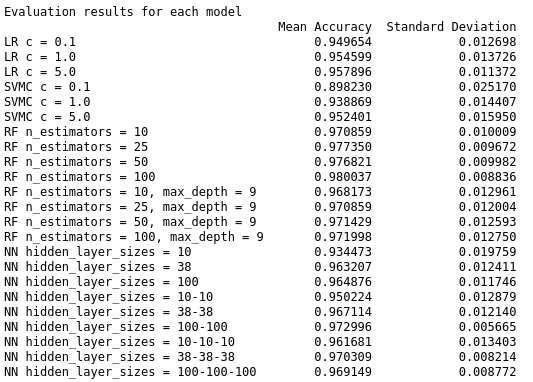
\includegraphics[scale=0.6]{img/eval-results.png}
    \caption{Resultado de la evaluación de los modelos.}
    \label{fig:eval-results}
\end{figure}

Podemos ver a simple vista que la mayoría de modelos, con distintas combinaciones de hiperparámetros, ofrecen unos \textbf{resultados} muy buenos, ya que el
porcentaje de \textit{accuracy} medio para todas las particiones de validación está muy cerca o por encima del 90\%. Además, las desviaciones
típicas de estos resultados nos indican que, de media, no existe una gran variabilidad entre los resultados que se obtienen para las particiones
de validación, si no que son bastante próximos.

Vamos a analizar ahora cada modelo de forma separada para intentar ver mejor cómo se comportan. Nos vamos a ayudar de las \textbf{curvas de aprendizaje},
las cuáles han sido obtenidas con una función muy parecida a esta \cite{bib:learning_curve}. Empecemos el análisis por el primer modelo, la
Regresión Logística Multinomial.

Podemos ver que este modelo ofrece unos resultados excelentes a pesar de ser solo un modelo lineal. Se puede ver que tiene aproximadamente
un porcentaje de \textit{accuracy} medio muy cercano o un poco superior al 95\%, lo cuál nos indica que lo hace bastante bien a pesar se ser
un modelo tan simple. Vemos que, a medida que aumenta el valor de $C$ (el hiperparámetro que controla el grado de regularización) los resultados
van mejorando, aunque tampoco es una mejora demasiado significativa. Vamos a estudiar brevemente las curvas de aprendizaje de este modelo para
ver cómo de bien lo hace:

\begin{figure}[H]
\centering
\begin{minipage}{.5\textwidth}
    \centering
    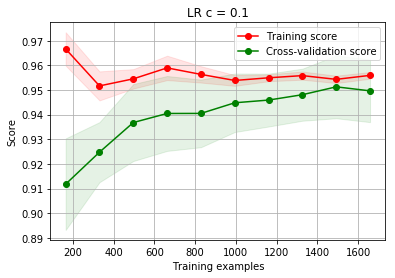
\includegraphics[scale=0.4]{img/lc-lr-c-01.png}
    \caption{Curva de aprendizaje del modelo de Regresión Logística con $C=0.1$.}
    \label{fig:lc-lr-c-01}
\end{minipage}%
\begin{minipage}{.5\textwidth}
    \centering
    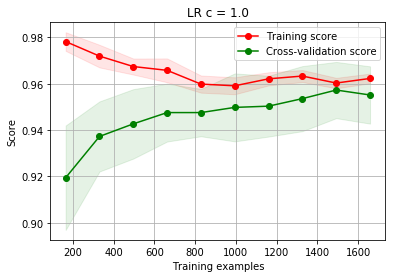
\includegraphics[scale=0.4]{img/lc-lr-c-1.png}
    \caption{Curva de aprendizaje del modelo de Regresión Logística con $C=1.0$.}
    \label{fig:lc-lr-c-1}
\end{minipage}
\end{figure}

\begin{figure}[H]
    \centering
    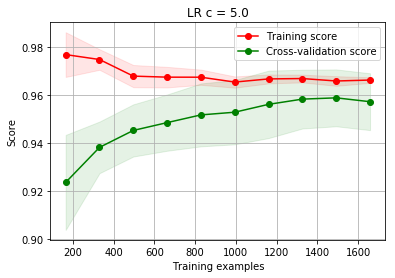
\includegraphics[scale=0.5]{img/lc-lr-c-5.png}
    \caption{Curva de aprendizaje del modelo de Regresión Logística con $C=5.0$.}
    \label{fig:lc-lr-c-5}
\end{figure}

En los 3 casos, podemos ver que es un modelo con \textbf{bajo sesgo}, ya que los resultados medios de \textit{accuracy} obtenidos para las particiones de
entrenamiento son muy buenos. Sin embargo, a medida que va aumentando el tamaño de la muestra de entrenamiento, la \textit{accuracy} de entrenamiento
va disminuyendo, lo cuál es normal ya que hay más ejemplos con los que ir probando. Por otra parte, parece que también es un modelo con \textbf{baja
varianza}, ya que a medida que va aumentando el tamaño de la muestra de entrenamiento, las diferencias entre los resultados de entrenamiento y de validación
van disminuyendo, hasta que al final casi han convergido. Parece que en general las 3 configuraciones de hiperparámetros ofrecen unos buenos
resultados, además de que son muy parecidos entre sí. La única diferencia es que, a medida que va aumentando el valor de $C$, la curva de validación
se va suavizando más y más. Sin embargo, en los 3 casos se puede observar una convergencia común entre los 1400 y los 1600 datos de entrenamiento,
lo cuál puede significar que el modelo no se beneficiaría de tener más datos de entrenamiento, ya que, al haber convergido las dos curvas, ha llegado
al máximo rendimiento que podría ofrecer para este problema, y exigirle más seguramente implicaría un empeoramiento de los valores de que se
obtendrían en validación.

El siguiente modelo que vamos a analizar es el SVM con \textit{kernel} RBF. Podemos ver en la figura \ref{fig:eval-results} que este modelo, en
general, es el que ofrece para la mayoría de configuraciones de hiperparámetros los peores resultados. Es el que
ofrece una peor \textit{accuracy} de media, ya que con $C = 0.1$ esta se queda cerca del 90\%, un valor muy inferior al resto de valores que se
pueden ver en la figura. A medida que aumenta el valor de $C$, sin embargo, se puede ver que los resultados obtenidos van mejorando, y la
variabilidad, la cuál viene dada por la desviación típica, también se ve reducida al compararla con la que teníamos inicialmente. El motivo de estos
resultados puede deberse a que no se haya ajustado correctamente el hiperparámetro $gamma$. Además, a mano es muy difícil encontrar una buena
combinación de éstos, con lo cuál los resultados obtenidos no serán siempre los mejores. A pesar de eso, con valores un poco más altos de $C$, los
resultados no parecen ser para nada malos, aunque se queda un poco lejos de la Regresión Logística Multinomial. Observemos ahora
las curvas para tener una mejor información de lo que está pasando:

\begin{figure}[H]
    \centering
    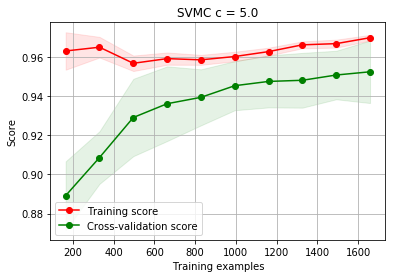
\includegraphics[scale=0.5]{img/lc-svm-c-5.png}
    \caption{Curva de aprendizaje del modelo SVM con $C=5.0$.}
    \label{fig:lc-svm-c-5}
\end{figure}

\begin{figure}[H]
\centering
\begin{minipage}{.5\textwidth}
    \centering
    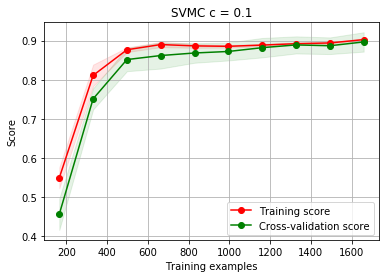
\includegraphics[scale=0.45]{img/lc-svm-c-01.png}
    \caption{Curva de aprendizaje del modelo SVM con $C = 0.1$.}
    \label{fig:lc-svm-c-01}
\end{minipage}%
\begin{minipage}{.5\textwidth}
    \centering
    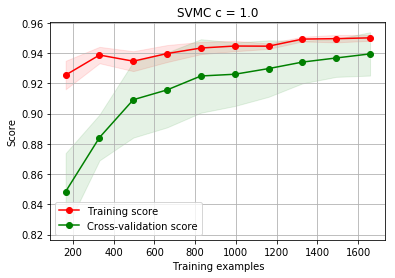
\includegraphics[scale=0.45]{img/lc-svm-c-1.png}
    \caption{Curva de aprendizaje del modelo SVM con $C=1.0$.}
    \label{fig:lc-svm-c-1}
\end{minipage}
\end{figure}

Podemos ver que el sesgo del modelo va cambiando en función del valor del hiperparámetro $C$. Si es más bajo, podemos ver que el modelo tiene \textbf{mucho
sesgo}, ya que el error de entrenamiento es bastante elevado, lo cuál implica un \textit{accuracy} más bajo, a pesar de que vaya mejorando a
medida que se le proporcionen más datos. En los otros casos, el sesgo sigue siendo más alto que por ejemplo el de Regresión Logística Multinomial
y se sigue manteniendo relativamente alto, lo cuál no quita el hecho de haya habido una mejora en éste, ya que se puede ver que es mucho menor
que el que teníamos inicialmente con un valor de $C = 0.1$. Además, parece que a medida que aumenta el tamaño de la muestra que se utiliza para
entrenar el modelo, el sesgo se va reduciendo, aunque llega un punto en el que se estanca y parece no mejorar mucho o muy poco.
En cuanto a la \textbf{varianza}, en este modelo podemos ver en general es muy baja, ya que los resultados obtenidos en validación están bastante
próximos a los que se obtienen en el entrenamiento. Además, igual que pasa con el sesgo, a medida que van aumentando la cantidad de datos en la
muestra de entrenamiento, más se reduce la varianza media. Sin embargo, tal y como pasa con el sesgo, llega un momento en el que casi ha convergido, con lo cuál, llegaría un punto en el que, por muchos datos que le suministráramos al modelo, no podría llegar a mejorar. A pesar de
eso, parece que con la configuración adecuada de hiperparámetros, tiene todavía cierto margen de mejora, aunque no sea mucho.

Pasemos ahora al Random Forest. Observando los resultados que se pueden ver en la figura \ref{fig:eval-results}, podemos apreciar claramente como
este modelo es el que ofrece los mejores resultados en general para todas las combinaciones de hiperparámetros que se han probado. Se puede ver que
el único modelo que se le acerca en cuanto a porcentaje medio de \textit{accuracy} son las Redes Neuronales, de las cuáles hablaremos más adelante.
Además, los valores medios de las desviaciones típicas son en general bastante buenos, lo cuál nos indica que hemos probado con un modelo robusto
capaz de ofrecer unos resultados muy buenos.

Se puede ver que, el Random Forest que se ha probado sin establecer una profundidad límite, ha dado resultados ligeramente mejores que aquel donde
hemos establecido que la profundidad máxima sea de 9 niveles. Sin embargo, como en el primer caso no se ha realizado ningún tipo de poda, no
podemos estar seguros de que no se haya producido sobreajuste en el modelo, lo cuál podría llevar a que los resultados obtenidos en la validación
sean mucho peores. Para ver un poco esto, vamos a estudiar brevemente las curvas de aprendizaje de las dos opciones, tanto sin límite de profundidad
como con límite.

\begin{figure}[H]
\centering
\begin{minipage}{.5\textwidth}
    \centering
    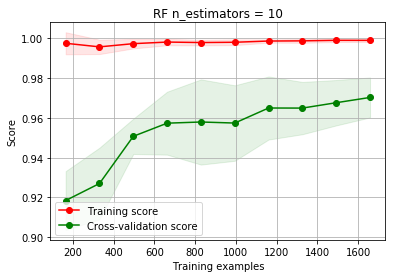
\includegraphics[scale=0.4]{img/lc-rf-n-10.png}
    \caption{Curva de aprendizaje de Random Forest con $n\_estimators=10$.}
    \label{fig:lc-rf-n-10}
\end{minipage}%
\begin{minipage}{.5\textwidth}
    \centering
    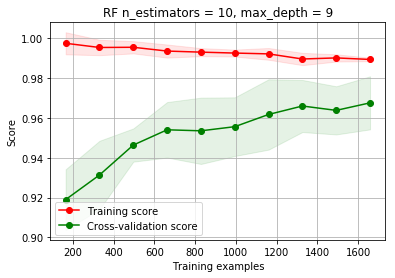
\includegraphics[scale=0.4]{img/lc-rf-n-10-d-9.png}
    \caption{Curva de aprendizaje de Random Forest con $n\_estimators=10$ y $max\_depth=9$.}
    \label{fig:lc-rf-n-10-d-9}
\end{minipage}
\end{figure}

\begin{figure}[H]
\centering
\begin{minipage}{.5\textwidth}
    \centering
    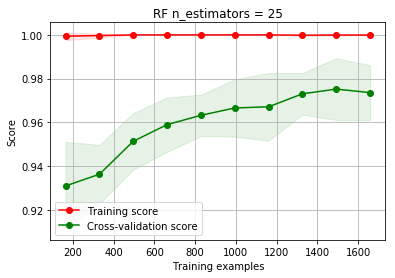
\includegraphics[scale=0.4]{img/lc-rf-n-25.png}
    \caption{Curva de aprendizaje de Random Forest con $n\_estimators=25$.}
    \label{fig:lc-rf-n-25}
\end{minipage}%
\begin{minipage}{.5\textwidth}
    \centering
    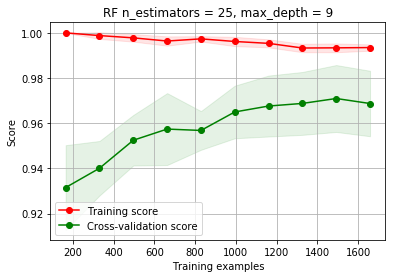
\includegraphics[scale=0.4]{img/lc-rf-n-25-d-9.png}
    \caption{Curva de aprendizaje de Random Forest con $n\_estimators=25$ y $max\_depth=9$.}
    \label{fig:lc-rf-n-25-d-9}
\end{minipage}
\end{figure}

\begin{figure}[H]
\centering
\begin{minipage}{.5\textwidth}
    \centering
    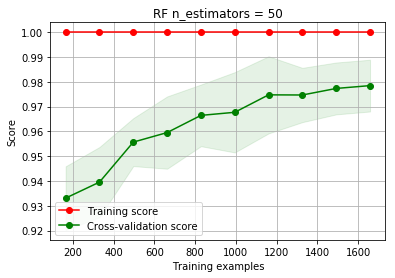
\includegraphics[scale=0.4]{img/lc-rf-n-50.png}
    \caption{Curva de aprendizaje de Random Forest con $n\_estimators=50$.}
    \label{fig:lc-rf-n-50}
\end{minipage}%
\begin{minipage}{.5\textwidth}
    \centering
    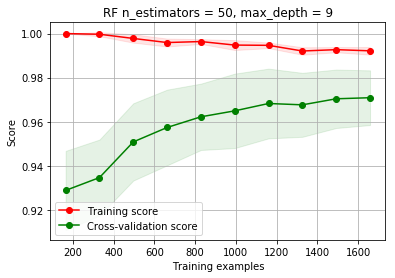
\includegraphics[scale=0.4]{img/lc-rf-n-50-d-9.png}
    \caption{Curva de aprendizaje de Random Forest con $n\_estimators=50$ y $max\_depth=9$.}
    \label{fig:lc-rf-n-50-d-9}
\end{minipage}
\end{figure}

\begin{figure}[H]
\centering
\begin{minipage}{.5\textwidth}
    \centering
    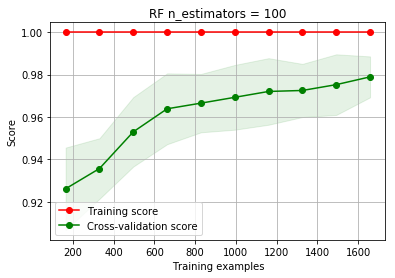
\includegraphics[scale=0.4]{img/lc-rf-n-100.png}
    \caption{Curva de aprendizaje de Random Forest con $n\_estimators=100$.}
    \label{fig:lc-rf-n-100}
\end{minipage}%
\begin{minipage}{.5\textwidth}
    \centering
    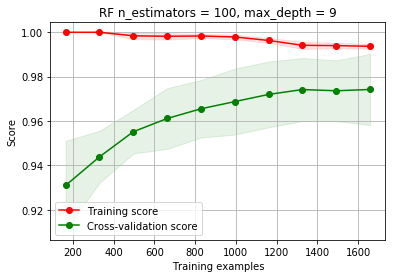
\includegraphics[scale=0.4]{img/lc-rf-n-100-d-9.png}
    \caption{Curva de aprendizaje de Random Forest con $n\_estimators=100$ y $max\_depth=9$.}
    \label{fig:lc-rf-n-100-d-9}
\end{minipage}
\end{figure}

Como ya sabíamos de antes, el modelo presenta un \textbf{sesgo muy bajo} o casi nulo. Esto se puede ver en que las tasas medias de \textit{accuracy} en las
particiones de entrenamiento son muy altas y que casi no hay error. También son modelos que presentan una \textbf{varianza relativamente baja}, ya que, a
medida que va aumentando la cantidad de datos con los que se entrena la muestra, se puede ver como la \textit{accuracy} de validación se va
acercando cada vez más y más a la de entrenamiento hasta situarse muy cerca de ésta. Por tanto, podemos ver que, a mayor cantidad de datos, mejor se
comporta el modelo. Por tanto, nos encontramos ante un modelo que es capaz de generar muy buenas generalizaciones cuantos más datos tiene.

Otro punto que es importante destacar es que los resultados que se pueden ver en las gráficas son bastante \textbf{parecidos}. Se puede ver como, aunque
la \textit{accuracy} media varía ligeramente entre la versión con tope de profundidad y la versión sin, las tasas de \textit{accuracy} medias
obtenidas en las particiones de validación son muy parecidas, lo cuál parece ser un buen indicio de que, al podar los árboles a priori, no perdemos
mucha capacidad de generalización, además de que los árboles resultantes serán muy posiblemente más simples.

Finalmente, pasemos a analizar las Redes Neuronales. Según los resultados que podemos observar en la figura \ref{fig:eval-results}, podemos ver que,
dependiendo de la arquitectura utilizada, vamos a obtener unos resultados u otros. Para arquitecturas con pocas unidades por capa, se puede ver
que los resultados son un poco peores en general, independientemente del número de capas ocultas que se estén utilizando. En cambio, al ir aumentando
el número de unidades por capa, vemos como los resultados van mejorando, acercándose incluso a los resultados que nos permitía obtener el Random
Forest. Al ir aumentando el número de capas ocultas también se ha producido una ligera mejora de los resultados. Sin embargo, hay que tener en
cuenta que, al no haber regularizado el modelo, al incrementar demasiado el número de capas y niveles se podrían dar casos de sobreajuste, lo
cuál haría que las generalizaciones fuesen mucho peores que los resultados obtenidos en los conjuntos de entrenamiento. Para comprobar si existe
o no sobreajuste, vamos a comparar las curvas de aprendizaje del modelo para cada configuración de unidades por capa:

\begin{figure}[H]
\centering
\begin{minipage}{.5\textwidth}
    \centering
    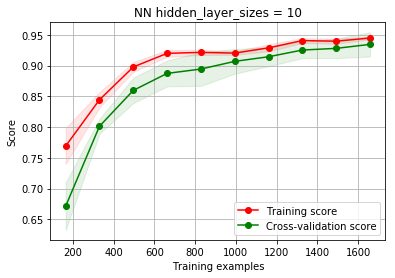
\includegraphics[scale=0.4]{img/lc-nn-10.png}
    \caption{Curva de aprendizaje del modelo de Neural Network con $hidden\_layer\_sizes=10$.}
    \label{fig:lc-nn-10}
\end{minipage}%
\begin{minipage}{.5\textwidth}
    \centering
    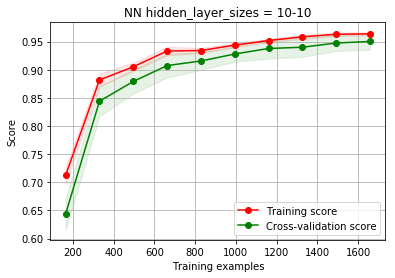
\includegraphics[scale=0.4]{img/lc-nn-10-10.png}
    \caption{Curva de aprendizaje del modelo de Neural Network con $hidden\_layer\_sizes=10-10$.}
    \label{fig:lc-nn-10-10}
\end{minipage}
\end{figure}

\begin{figure}[H]
    \centering
    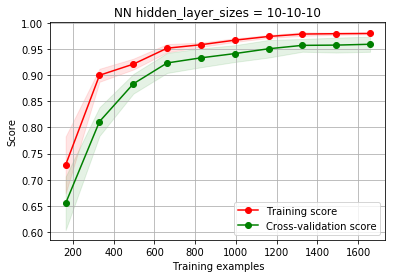
\includegraphics[scale=0.5]{img/lc-nn-10-10-10.png}
    \caption{Curva de aprendizaje del modelo de Neural Network con $hidden\_layer\_sizes=10-10-10$.}
    \label{fig:lc-nn-10-10-10}
\end{figure}

Para esta configuración de unidades 10 unidades por capa, podemos ver que, con una cantidad de datos pequeña existe un \textbf{sesgo altísimo}, lo cuál hace
que el modelo tenga unos resultados terribles luego en la validación. A medida que va aumentando el número de elementos de la muestra de
entrenamiento, el sesgo se va reduciendo, lo cuál nos indica que, si hubiéramos intentado aplicar una Red Neuronal con estas mismas arquitecturas
y este mismo número de unidades por capa con la muestra de entrenamiento que teníamos al principio, hubiésemos obtenido unos resultados terribles
en genera. Es importante destacar, no obstante, que existe \textbf{muy poca varianza}, ya que los resultados medios obtenidos con las particiones de
validación son muy cercanos a los obtenidos con las particiones de entrenamiento.

\begin{figure}[H]
\centering
\begin{minipage}{.5\textwidth}
    \centering
    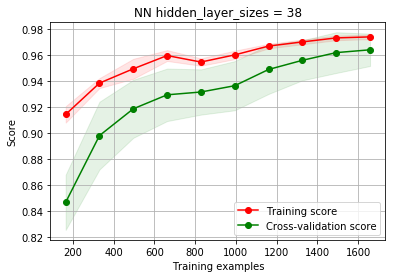
\includegraphics[scale=0.4]{img/lc-nn-38.png}
    \caption{Curva de aprendizaje del modelo de Neural Network con $hidden\_layer\_sizes=38$.}
    \label{fig:lc-nn-38}
\end{minipage}%
\begin{minipage}{.5\textwidth}
    \centering
    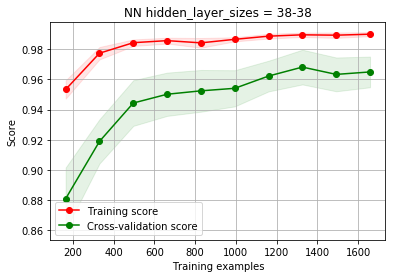
\includegraphics[scale=0.4]{img/lc-nn-38-38.png}
    \caption{Curva de aprendizaje del modelo de Neural Network con $hidden\_layer\_sizes=38-38$.}
    \label{fig:lc-nn-38-38}
\end{minipage}
\end{figure}

\begin{figure}[H]
    \centering
    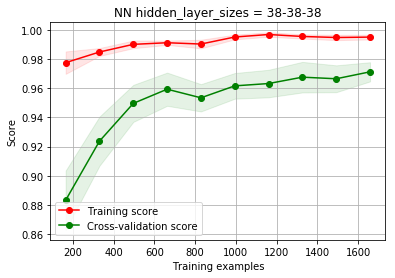
\includegraphics[scale=0.5]{img/lc-nn-38-38-38.png}
    \caption{Curva de aprendizaje del modelo de Neural Network con $hidden\_layer\_sizes=38-38-38$.}
    \label{fig:lc-nn-38-38-38}
\end{figure}

Analizando ahora las curvas de aprendizaje de estas arquitecturas con 38 unidades por capa (un poco más del doble de características de las
que disponemos al entrenar los modelos), vemos como el \textbf{sesgo} es muchísimo \textbf{menor} que en el caso contrario, incluso para pocos datos. 
Además, podemos ver que, a medida que aumentamos los datos de entrenamiento, este se va reduciendo incluso más, hasta llegar a un punto en el que
\textbf{converge} en torno al 0.98.

Aquí sí que hay un poco \textbf{más de varianza} respecto al modelo anterior, pero, al igual que sucede con
el sesgo, ésta se va reduciendo a medida que hay más datos para entrenar el modelo. Si dispusiéramos de una cantidad de datos pequeña para entrenar el
modelo, estaríamos en un caso de sobreajuste, ya que hay muchísima diferencia entre los resultados obtenidos en entrenamiento y los obtenidos en validación.

También, a mediada que se va aumentando el número de capas, parece que es más difícil que los resultados de entrenamiento y los de validación se acerquen
mucho, ya que parece que se quedan separados por una diferencia que en un principio no es muy significativa, pero haría que nunca se pudiesen conseguir los
mismos resultados en las particiones de validación que en las de entrenamiento. Por tanto, existe cierto riesgo de sobreajuste, ya que podría darse
que, al tener más datos, los resultados en los conjuntos de validación fuesen mucho peores.

\begin{figure}[H]
\centering
\begin{minipage}{.5\textwidth}
    \centering
    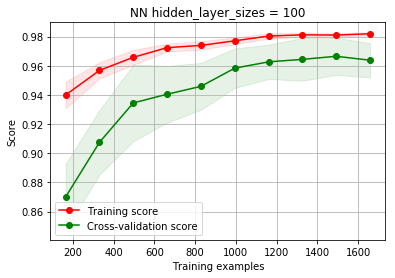
\includegraphics[scale=0.4]{img/lc-nn-100.png}
    \caption{Curva de aprendizaje del modelo de Neural Network con $hidden\_layer\_sizes=100$.}
    \label{fig:lc-nn-100}
\end{minipage}%
\begin{minipage}{.5\textwidth}
    \centering
    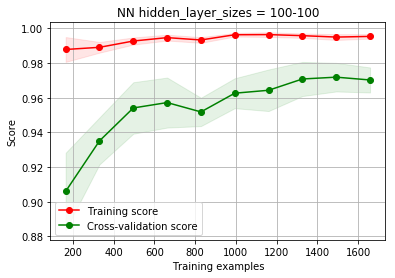
\includegraphics[scale=0.4]{img/lc-nn-100-100.png}
    \caption{Curva de aprendizaje del modelo de Neural Network con $hidden\_layer\_sizes=100-100$.}
    \label{fig:lc-nn-100-100}
\end{minipage}
\end{figure}

\begin{figure}[H]
    \centering
    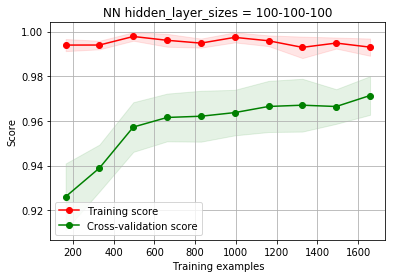
\includegraphics[scale=0.5]{img/lc-nn-100-100-100.png}
    \caption{Curva de aprendizaje del modelo de Neural Network con $hidden\_layer\_sizes=100-100-100$.}
    \label{fig:lc-nn-100-100-100}
\end{figure}

Para este ultimo modelo, vemos que sucede algo parecido que en el caso contrario en cuanto a sesgo y varianza. También vemos que, de nuevo, al
complicar la arquitectura, se complica que los resultados de entrenamiento y de validación se acerquen, lo cuál, de nuevo, podría provocar sobreajuste
y a obtener unos peores resultados con un mayor número de datos.

\newpage

\section{\textsc{Elección de los mejores modelos}}

Una vez analizados todos los modelos, utilizando \textbf{cross-validation} y diversos hiperparámetros para cada uno de ellos, vamos a
comentar cuáles han sido los que han obtenido los mejores resultados y porqué. Para ello nos vamos a ayudar de las métricas obtenidas
anteriormente, es decir, utilizaremos tanto la tabla que nos muestra la \textbf{media de aciertos} y \textbf{desviaciones típicas}, como
las \textbf{curvas de aprendizaje} de cada uno de los modelos \ref{fig:eval-results}.

Observando los resultados obtenidos, tenemos que el Random Forest con un $n\_estimators = 50$ es el que mayor porcentaje de acierto ha
tenido, con un 97.8470\%; mientras que el que menor desviación típica ha conseguido es el MLPClassifier con un $hidden\_layer\_sizes =
(100-100)$, con un valor de 0.005839. No obstante, podemos ver que el porcentaje de acierto de la mayoría de clasificadores es muy alto,
entre el 96\% y el 97\%, y los valores de las desviaciones típicas también son bastante bastante bajos, entre el 0.005 y el 0.02; así que
tendremos que tener en cuenta más cosas a parte de estas.

Vamos a \textbf{analizar las gráfica}s de los modelos para ver si encontramos algunos detalles más significativos en ellas:

\begin{itemize}[label=\textbullet]
    \item Si empezamos por las de Regresión Logística, vemos que las curvas son bastante suaves para los parámetros de $C = 1.0$ y $C = 5.0$ y a
    medida que aumenta el tamaño del conjunto de entrenamiento, la clasificación va mejorando (aunque debido a la convergencia entre las dos líneas
    podemos decir que, por más muestras de entrenamiento que tengamos, no va mejorar mucho mas) y el sobreajuste se reduce.
    \item En cuanto al SVM, podemos ver que las gráficas no son malas, es decir, son bastante suaves y apenas tienen sobreajuste, pero los
    resultados a los que se está llegando son los peores en comparación con el resto.
    \item En el Random Forest podemos ver que las curvas van aumentando suavemente a medida que el número de evaluaciones es más grande; y lo que es
    más importante, pueden seguir mejorando agregando más muestras de entrenamiento. Por otra parte, el valor del \textit{Training score} ronda
    siempre el 1, lo que puede ser un síntoma de sobreajuste si la varianza con los datos de validación es alta. Además de eso, si los árboles
    no están podados, hay más riesgo de sobreajuste, tal y como se ha dicho antes.
    \item Las gráficas de las Redes Neuronales son muy similares a las del Random Forest, con la única diferencia de que los valores del
    \textit{Training score} son un poco más bajos y más parecidos, en general, a los obtenidos en los conjuntos de validación. Sin embargo,
    tal y como se comentó anteriormente, existe cierto riesgo al sobreajuste, al no haber regularizado el modelo.
\end{itemize}

Gracias a este análisis, podemos decir que el SVM no va a ser uno de nuestros mejores modelos, porque nos ha ofrecido los resultados más
pobres en cuanto a la precisión y la desviación típica, y sus gráficas tampoco eran las mejores. Aun así, este no es un mal clasificador
(hemos podido comprobar que su porcentaje de acierto suele ser mayor de 90), pero lo tenemos que descartar porque tenemos al resto que
están un paso por delante.

Entre los tres modelos restantes nos vamos a quedar con la \textbf{Regresión Logística Multinomial} y con el \textbf{Random Forest}. Estos
clasificadores son bastante simples y han obtenido unos muy buenos resultados en general, incluso siendo uno de ellos un modelo lineal. No hemos
escogido las Redes Neuronales debido a que, a pesar de los sofisticadas que son y de que en general han obtenido unos buenos resultados,
el hecho de que su arquitectura sea más compleja que la del resto de modelos y a que son más lentas en general a la hora de ser entrenadas no
justifica unas ganancias muy pobres o casi nulas respecto a otros modelos que obtienen mejores resultados siendo más rápidos en general.

\section{\textsc{Ajuste de las técnicas seleccionadas}}

\subsection{Regresión Logística}

Este modelo hemos visto que no ofrecía las mejores soluciones (aunque no se quedaba lejos de ellas), pero como es significativamente más
rápido que las Redes Neuronales, vamos a intentar \textbf{ajustar sus hiperparámetros} al máximo para conseguir mejorar sus resultados. Esto lo
haremos creando un \textbf{grid} con los distintos valores que le podremos asignar a nuestro algoritmo, y posteriormente ejecutándolo para cada uno
de ellos. Este es código que crea el grid y el modelo de Regresión Logística:

\begin{lstlisting}
# Crear grid de hiperparametros que se van a probar
param_grid_lr = [{'C': np.linspace(0.1, 1.0, 10),
                  'multi_class': ['multinomial'],
                  'solver': ['newton-cg'],
                  'random_state': [1]}]

# Crear modelo de regresion logistica
mlr = LogisticRegression()
\end{lstlisting}

Para el parámetro $C$ generamos una muestra de tamaño 10 con valores que van del 0.1 hasta el 1.0. Éste será el único hiperparámetro que
cambie, ya que $multi\_class$ sólo podrá adoptar el valor $'multinomial'$ y $solver$ sólo tendrán el valor \textit{`newton-cg'}. El primero de
ellos es porque estamos en un problema multiclase, y el segundo de ellos porque ofrece una mejor minimización de la función cuadrática. El
último hiperparámetro $random\_state$ es la semilla para los aleatorios, así que no es muy importante.

A continuación, utilizaremos el método \textbf{\textit{GridSearchCV}}\cite{GridSearchCV} para realizar una búsqueda exhaustiva entre todos
los valores de los parámetros especificados y quedarnos con el mejor. Este método implementa funciones como $fit$ o $score$ que nos
ayudarán a evaluarlo, y parámetros como \textit{best\_estimator\_} que nos dirá cuál ha sido el mejor modelo de todos. Esta evaluación, al igual
que las anteriores, también se realizará mediante \textit{cross-validation} (implementada por la propia función). Veamos el código donde
aplicamos \textit{GridSearchCV}:

\begin{lstlisting}
# Crear GridSearch con Cross Validation para determinar
# la mejor combinacion de parametros
grid_search = GridSearchCV(mlr, param_grid=param_grid_lr, cv=cv,
                           scoring='accuracy')

# Aplicar GridSearch para obtener la mejor combinacion de hiperparametros
grid_search.fit(X_train, y_train)

# Obtener indice de la mejor media de test
best_idx = np.argmax(grid_search.cv_results_['mean_test_score'])

\end{lstlisting}

El resultado de ejecutar todo esto ha sido el siguiente:

\begin{figure}[H]
    \centering
    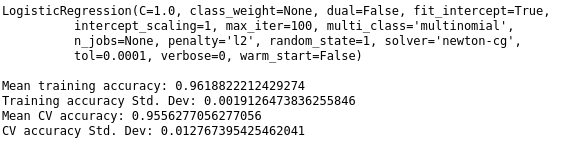
\includegraphics[scale=0.8]{img/gs-lr.png}
    \caption{Resultados de \textit{GridSearch} sobre la Regresión Logística.}
    \label{fig:gs-lr}
\end{figure}

Como podemos observar, el método ha seleccionado como valor para el hiperparámetro \textbf{C = 0.5}, el cual no habíamos prefijado en las pruebas
iniciales (0.1, 1.0, 5.0). Este valor está bastante bien estimado, ya que valores más bajos, como 0.1, hacen que la regularización sea bastante
floja, mientras que con valores más altos, como 5.0, se puede llegar a producir \textit{underfitting}, ya que se habrá regularizado tanto que el
modelo será demasiado simple. Lo lógico sería elegir valores por este rango de 0.5-1.0 aproximadamente, ya que son los que evitan los problemas
anteriores.

Si nos paramos a analizar tanto la \textbf{precisión} como la \textbf{desviación típica}, los valores obtenidos con este nuevo hiperparámetro son peores, a
priori, que los que teníamos anteriormente para este modelo. Tenemos que tener en cuenta que este valor es calculado en \textit{cross-validation}, y los
valores más malos vienen a partir del tercer decimal. Lo que nos lleva a decir que este modelo está mejor ajustado es que el valor de $C$ ha sido
seleccionado de forma que se regulariza en una medida apropiada para conseguir buenos resultados, en vez de probando a mano cuál de los valores
funciona mejor.

Concluimos que, pese a no haber mejorado los resultados iniciales, el modelo sigue clasificando bastante bien. No obstante, \textbf{no lo
seleccionaremos} como nuestro modelo final, ya que los clasificadores Random Forest lo hacen mejor con una complejidad similar (e incluso las
Redes Neuronales, aunque habría que estudiarlo en términos de eficiencia y simplicidad), y aún no hemos estudiado sus hiperparámetros y si
estos pueden hacer que mejore.

\subsection{Random Forest}

Es el turno de Random Forest, el modelo que mejores resultados ha obtenido en cuanto a precisión media y a varianza, que no tenía unas
malas curvas de aprendizaje, y que no es tan rápido como los SVM pero tienen una complejidad y tiempo de cómputo aceptable. Para intentar
mejorar, o \textbf{encontrar los hiperparámetros} que mejor se ajustan a este modelo vamos a utilizar la misma técnica de antes, el
\textit{GridSearchCV}. En este caso, el grid y el modelo Random Forest se crea de la siguiente forma:

\begin{lstlisting}
# Crear grid de hiperparametros que se van a probar
param_grid_rf = [{'n_estimators': np.linspace(50,500,10,dtype=np.int),
                  'max_depth': np.linspace(5, 15, 6, dtype=np.int),
                  'random_state': [1]}]

# Crear modelo de Random Forest
rf = RandomForestClassifier()

\end{lstlisting}

Para el hiperparámetro $n\_estimators$, que determina el número de árboles, generamos una muestra de tamaño 10 con valores que van desde el
50 hasta el 500; y para $max\_depth$, que determina la profundidad de los árboles, generaremos otra muestra, en este caso de tamaño 6 y con
valores que van desde el 5 hasta el 15. El último hiperparámetro también será $random\_state$, que al igual que antes, es la semilla para
los aleatorios.

Como la técnica para realizar la búsqueda de los mejores valores es la misma que la utilizada anteriormente en Regresión Logística, no la
vamos a volver a explicar, simplemente pasemos a ver los resultados que nos ha dado:

\begin{figure}[H]
    \centering
    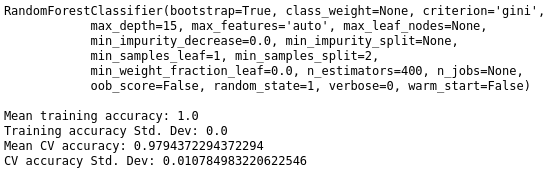
\includegraphics[scale=0.6]{img/gs-rf.png}
    \caption{Resultados de \textit{GridSearch} sobre Random Forest.}
    \label{fig:gs-rf}
\end{figure}

Podemos ver que el mejor valor que ha encontrado para el \textit{\textbf{n\_estimators}} ha sido \textbf{400}, es decir, más alto 
(más número de árboles) que en elmodelo inicial, lo cual nos dice que tendríamos que haber probado con un número de árboles superior a los 
prefijados. Por otro lado, para \textit{\textbf{max\_depth}} el valor que ha obtenido ha sido \textbf{15}, es decir, a diferencia de la ejecución inicial nos asigna 
un valor de profundidad límite. También hay que tener en cuenta que nosotros intentamos poner una profundidad de 9 en esas ejecuciones y 
los resultados no eran tan buenos como con estos hiperparámetros.

En cuanto a las medias en la \textbf{precisión} y en la \textbf{desviación típica}, también son valores muy similares a los obtenidos en la ejecución
inicial. Sin embargo, son valores similares a los árboles sin una profundidad determinada, es decir, que hemos conseguido un porcentaje de
acierto y una desviación típica tan buena como los anteriores pero con una \textbf{profundidad de árbol limitada}. También hay que tener en cuenta
el número de árboles utilizados, pero si se ha seleccionado este modelo como el mejor, es porque merece más la pena tener un mayor número
de árboles con una profundidad limitada que tener pocos árboles con mucha profundidad. Esto se debe a que los primeros se han podado a
priori y los segundos, al no haber especificado una profundidad máxima, no se han podado, con lo cuál son más sensibles al sobreajuste.
Además, tener más árboles, y que además estén podados, puede hacer que la generalización del modelo sea aún mejor.

Como conclusión, decir que \textbf{nos vamos a quedar con este último modelo} de Random Forest obtenido como el mejor clasificador para el problema.
Ya vimos anteriormente que los Random Forest eran el mejor modelo (o de los mejores) en la ejecución inicial, y como acabamos de comprobar,
ajustando los modelos no hay ninguno que llegue a su nivel. Es más, ajustando el modelo hemos conseguido unos parámetros que mejoran los
asignados en un principio, así que partiremos de estos para realizar la evaluación final.

\section{\textsc{Evaluación del mejor modelo}}

Una vez elegido el modelo y ajustados los hiperparámetros, vamos a realizar la evaluación final. Para ello nos ayudaremos de dos cosas: 
\begin{enumerate}
    \item El conjunto de test, el cuál habíamos obtenido al principio mediante \textit{hold-out}.
    \item Un modelo de referencia llamado \textbf{\textit{DummyClassifier}}\cite{DummyClassifier}, el cuál utiliza reglas simples y que está
    especialmente diseñado para ser comparado con otras técnicas reales de clasificación (no se utiliza para problemas reales).
\end{enumerate}

El código para generar este clasificador de referencia es el siguiente:

\begin{lstlisting}
# Creamos modelo de prueba y lo entrenamos
dummy = DummyClassifier()
dummy.fit(X_train, y_train)

# Predecir valores con dummy
y_predicted_dummy = dummy.predict(X_test)
\end{lstlisting}

Podemos observar que estamos utilizando el clasificador con los parámetros por defecto. Entre estos tenemos uno llamado $strategy$, que por defecto
tiene el valor $'stratified'$, el cual genera predicciones aleatorias respetando la distribución de clases del conjunto. Los otros dos atributos que
tenemos son el $random\_state$, que ya vimos para que sirve, y otro llamado $constant$, que sólo afectará si el parámetro $strategy$ adopta un
determinado valor (y no es nuestro caso).

Posteriormente, vamos a entrenar nuestro mejor modelo. Como estamos utilizando el que acabamos de ajustar y hemos clasificado como el mejor, no vamos a
volver a explicar cómo se ha hecho. Simplemente, recordar que hemos utilizado un \textbf{Random Forest Classifier} con los hiperparámetros ajustados a 400 árboles con una
profundidad máxima de 15.

A continuación, pasemos a la evaluación del modelo y a analizar los resultados obtenidos. Para ello vamos a mostrar las siguientes métricas para cada
uno de los dos modelos: $accuracy$, $recall$ y $precision$. Lo realizaremos gracias a las siguientes líneas de código:

\begin{lstlisting}
# Obtener metricas
dummy_score = accuracy_score(y_test, y_predicted_dummy)
rf_score = accuracy_score(y_test, y_predicted_rf)

dummy_recall = recall_score(y_test, y_predicted_dummy,
                            average='macro')
rf_recall = recall_score(y_test, y_predicted_rf,
                         average='macro')

dummy_precision = precision_score(y_test, y_predicted_dummy,
                                  average='macro')
rf_precision = precision_score(y_test, y_predicted_rf,
                               average='macro')
\end{lstlisting}

Los parámetros que les pasamos son las etiquetas que esperamos obtener, las etiquetas que ha predicho cada uno de los modelos y, con
$average$, el tipo de medias que obtendremos. En nuestro caso, con el valor $'macro'$, obtendremos la media de los de los resultados obtenidos
con esa métrica para cada clase. Los resultados han sido los siguientes:

\begin{figure}[H]
    \centering
    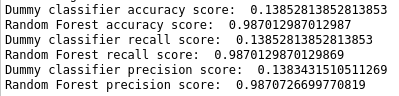
\includegraphics{img/model-comp-scores.png}
    \caption{Comparativa de métricas para evaluar el mejor modelo.}
    \label{fig:model-comp-scores}
\end{figure}

A simple vista nos damos cuenta de que un modelo aleatorio como el Dummy no es capaz de clasificar este problema correctamente. Podemos
ver que ha obtenido unos resultados muy malos (simplemente con observar el $13\%$ aproximado para los tres parámetros a estudiar, ya nos
dice que este problema tiene una complejidad a la hora de clasificar).

En cuanto a los resultados que ha obtenido el Random Forest, no tienen nada que ver con los del Dummy. Las predicciones han llegado a un
$98.701\%$ tanto en \textit{accuracy}, como en \textit{recall} (es decir, la tasa de aciertos o tasa de verdaderos positivos), y como en
\textit{precision} (verdaderos positivos entre todo el conjunto de positivos), y por tanto, comete un \textbf{1.3\% de error}. Estos
valores son mejores que los que obtuvimos anteriormente, al ajustar el modelo con \textit{cross-validation}. Esto es muy importante, ya
que estamos comprobando que el ajuste lo hemos realizado correctamente y, pese que los resultados cuando lo evaluamos en su momento fueron
peores, con un test más grande comprobamos que los hiperparámetros fueron elegidos correctamente.

Vamos a profundizar más en el análisis de este modelo sacando la matriz de confusión, para comprobar que parámetros obtenidos son
correctos y dónde se han cometido los fallos:

\begin{figure}[H]
    \centering
    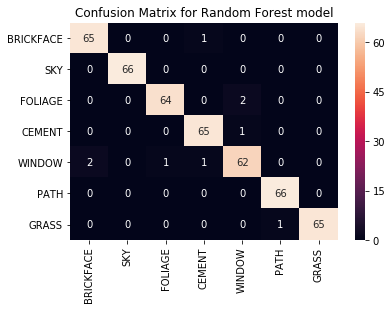
\includegraphics[scale=0.7]{img/confusion-matrix.png}
    \caption{Matriz de confusión de nuestro modelo ajustado.}
    \label{fig:confusion-matrix}
\end{figure}

Antes de analizarla, vamos a explicar que significa y que representa cada uno de sus valores. La \textbf{matriz de confusión} nos permite ver más
detalladamente el rendimiento de un algoritmo a través de sus dos ejes. El horizontal representa los valores reales de las clases;
y el vertical representa los valores predichos.

Si hubiésemos obtenido la matriz diagonal, el modelo tendría una precisión del $100\%$. En nuestro caso vemos que ha estado muy cerca de
conseguirlo, ya que únicamente \textbf{ha fallado en 6 de los 462 casos totales}. Donde más ha fallado ha sido al clasificar las ventanas
(\textit{WINDOW}), en la cuales ha puesto que 2 son ladrillos (\textit{BRICKFACE}) y una como cemento (\textit{CEMENT}). Esto quizás se
deba a que la ventana esté situada en una pared de ladrillos u hormigón y el clasificador, al ver los parámetros de esta, lo haya
entendido como tal. También encontramos un error al clasificar una hierba (\textit{GRASS}) como follaje (\textit{FOLIAGE}), otro al
clasificar un follaje (\textit{FOLIAGE}) como ventana (\textit{WINDOW}) y un último error al clasificar cemento (\textit{CEMENT}) como
hierba (\textit{GRASS}).

Estos errores probablemente también se deban a la misma razón comentada anteriormente. Decimos esto porque, teniendo en cuenta que no
hemos reducido dimensionalidad y tampoco le hemos aplicado PCA a los datos (simplemente hemos eliminado una variable constante), el ``fallo'' 
esté determinado por la propia imagen. Con esto nos referimos a que es un problema de la vida real, y los datos pueden contener ruido
provocado, o bien, porque la imagen no sea lo suficientemente representativa, o porque simplemente necesitemos más atributos que nos
permitan distinguir mejor entre clases.

Pese a comentar estos errores uno a uno no quiere decir que el modelo sea malo. Todo lo contrario, que hayamos podido enumerar los errores
entre 462 datos nos da una idea de lo bien que ha clasificado y de los pocos errores que ha cometido.

Otra métrica que vamos a analizar sobre este modelo va a ser su \textbf{curva de aprendizaje}. Vamos a ver primero la gráfica y
posteriormente pasaremos a comentarla:

\begin{figure}[H]
    \centering
    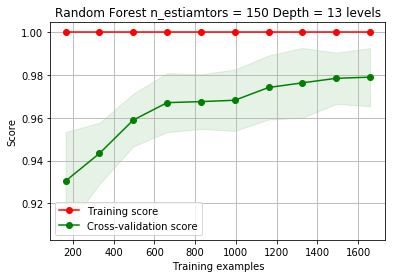
\includegraphics[scale=0.75]{img/lc-rf.png}
    \caption{Curva de aprendizaje de nuestro modelo ajustado.}
    \label{fig:lc-rf}
\end{figure}

Podemos ver que al principio, cuando tenemos pocos ejemplos de entrenamiento, la precisión entre los datos del \textit{Training} y del
\textit{Cross-validation} es muy diferente (tenemos una varianza muy alta). Sin embargo, a medida que vamos aumentando la cantidad de
ejemplos con los que entrenar, las líneas se empiezan a emparejar, ya que el modelo puede generalizar mucho mejor. La evolución de la curva
\textit{Cross-validation} es ascendente y bastante suave, lo que significa que el modelo aún tiene margen de mejora en caso de disponer de
más ejemplos de entrenamiento. El único inconveniente está en el sobreajuste debido a que, pese a tener curva muy buena como acabamos de
explicar, la precisión de entrenamiento (siempre vale 1.0) es ligeramente mayor que en la validación.

\newpage

\section{\textsc{Conclusiones}}

El objetivo de este trabajo era el de evaluar distintas técnicas para clasificar unas imágenes, extraídas del UCI Machine Learning
Repository, según el tipo de material que veamos en ellas. Para realizar esta clasificación hemos dado los siguientes pasos.

Primero hemos \textbf{analizado y modificado los datos}, unificando los dos ficheros proporcionados, realizando nuestra propia división en
\textit{training} y \textit{test}. Nos hemos dado cuenta de que no nos falta ningún valor en el conjunto y que nos sobra un atributo, que
era constante para todos los datos. No hemos eliminado las correlacionadas para evitar eliminar información útil.

Hemos \textbf{analizado todos los modelos}, comentando cómo funcionan, sus funciones de pérdida, si utilizan regularización y cuál, y algunos
detalles más específicos de cada uno. La evaluación de cada una de las técnicas la hemos realizado mediante las métricas
\textit{accuracy}, \textit{recall} y \textit{precision}, y la técnica de validación cruzada a la hora de entrenar. Gracias a esto
conseguimos un modelo que se ajuste de una forma generalizada a la naturaleza del conjunto de datos.

Cuando los hemos \textbf{evaluado y comparado}, nos hemos dado cuenta de que todos los modelos que hemos elegido ofrecen unos resultados muy buenos 
(casi todos por encima del 90\% de precisión) y con una variabilidad muy baja. Después hemos visto sus curvas de aprendizaje, en las que pudimos
ver cómo la Regresión Logística tenía una varianza y un sesgo bajos, teniendo en cuenta que es un modelo lineal; que el SVM tenía bastante sesgo
cuando el valor del parámetro $C$ era bajo y que además era el que peor precisión ha cometido a la hora de clasificar; que el Random Forest
ha obtenido los mejores resultados y además, sus gráficas tienen un sesgo prácticamente nulo y una varianza relativamente baja, la cual 
iba disminuyendo a medida que se aumentaban el número de ejemplos para entrenar; y por último, unas Redes Neuronales que ofrecían unos resultados
bastante similares a los del modelo anterior con la diferencia de que el sesgo era mucho más alto (aunque ha ido mejorando a medida que aumentábamos el
número de unidades por capa) y que son mucho más complejas. Una vez analizado esto, pasamos a seleccionar los mejores modelos.

Las técnicas que hemos seleccionado como las mejores han sido \textbf{Regresión Logística} y \textbf{Random Forest}. La primera porque,
con unos hiperparámetros prefijados por nosotros obtuvimos muy buenos resultados y no es una técnica tan compleja como las Redes
Neuronales. Las Redes Neuronales obtuvieron mejor resultado, pero con una diferencia no lo suficientemente significativa como para
compensar su complejidad. En cuanto al Random Forest, obtuvimos los mejores resultados sin apenas ajustar los modelos (únicamente probamos
a limitar la profundidad a 9). Sus curvas de aprendizaje no eran las mejores, sin embargo, no es un modelo tan complejo como el anterior,
así que merecía la pena intentar ajustarlo mejor.

Posteriormente, hemos \textbf{ajustado estas dos técnica}s mencionadas anteriormente. En Regresión Logística, hemos conseguido un mejor ajuste del
hiperparámetro $C$ (con un valor de 0.5), que evita una fuerte regularización o que aparezca el sobreajuste. No obstante, en términos de
precisión y desviación típica no ha mejorado al modelo inicial (95.5\% y 0.012 respectivamente), por lo que no lo seleccionaremos como el
mejor. En cuanto al Random Forest, hemos conseguido ajustar un valor de profundidad $max\_depth = 15$ pese a que el número de árboles que
ha elegido es mayor al que asignamos inicialmente $n\_estimators = 400$. Los valores de precisión y desviación típica son similares al
modelo inicial (97.9\% y 0.010 respectivamente), aunque hay que tener en cuenta que los iniciales se obtuvieron sin una profundidad
determinada.

Por último, hemos pasado a \textbf{evaluar el mejor modelo} (el Random Forest) a través del conjunto de test reservado
al principio y un DummyClassifier. Gracias a esta evaluación y al posterior análisis, pudimos comprobar que, tanto la técnica elegida como
el ajuste de sus hiperparámetros, lo hicimos bastante bien. Entre las 462 muestras sólo obtuvimos 6 errores. No podemos confirmar que esta
sea la mejor técnica, pero gracias a todo este análisis, es bastante apropiado para resolver nuestro problema.

\newpage

% Pagina de bibliografia
\begin{thebibliography}{25}

\bibitem{bib:uci-repo}
UCI. \textit{Image segmentation}
\\\url{http://archive.ics.uci.edu/ml/datasets/image+segmentation}

\bibitem{logistic-regression}
Scikit-Learn. \textit{LogisticRegression}
\\\url{https://scikit-learn.org/stable/modules/generated/sklearn.linear_model.LogisticRegression.html}

\bibitem{svc}
Scikit-Learn. \textit{SVC}
\\\url{https://scikit-learn.org/stable/modules/generated/sklearn.svm.SVC.html#sklearn.svm.SVC}

\bibitem{random_forest}
Scikit-Learn. \textit{RandomForestClassifier}
\\\url{https://scikit-learn.org/stable/modules/generated/sklearn.ensemble.RandomForestClassifier.html#sklearn.ensemble.RandomForestClassifier}

\bibitem{neural_network}
Scikit-Learn. \textit{MLPClassifier}
\\\url{https://scikit-learn.org/stable/modules/generated/sklearn.neural_network.MLPClassifier.html#sklearn.neural_network.MLPClassifier}

\bibitem{scaler}
Scikit-Learn. \textit{StandardScaler}
\\\url{https://scikit-learn.org/stable/modules/generated/sklearn.preprocessing.StandardScaler.html}

\bibitem{pca}
Scikit-Learn. \textit{PCA}
\\\url{https://scikit-learn.org/stable/modules/generated/sklearn.decomposition.PCA.html}

\bibitem{bib:learning_curve}
Scikit-Learn. \textit{plot\_learning\_curve}
\\\url{https://scikit-learn.org/stable/auto_examples/model_selection/plot_learning_curve.html#sphx-glr-auto-examples-model-selection-plot-learning-curve-py}

\bibitem{GridSearchCV}
Scikit-Learn. \textit{GridSearchCV}
\\\url{https://scikit-learn.org/stable/modules/generated/sklearn.model_selection.GridSearchCV.html}

\bibitem{DummyClassifier}
Scikit-Learn \textit{DummyClassifier}
\\\url{https://scikit-learn.org/stable/modules/generated/sklearn.dummy.DummyClassifier.html}

\bibitem{bib:recall}
Scikit-Learn. \textit{recall\_score}
\\\url{https://scikit-learn.org/stable/modules/generated/sklearn.metrics.recall_score.html}

\bibitem{bib:precision}
Scikit-Learn. \textit{precision\_score}
\\\url{https://scikit-learn.org/stable/modules/generated/sklearn.metrics.precision_score.html}

\bibitem{bib:normalize}
\textit{Should I normalize/standardize/rescale the data?}
\\\url{http://www.faqs.org/faqs/ai-faq/neural-nets/part2/}

\bibitem{bib:pipeline}
Scikit-Learn. \textit{5.1. Pipelines and composite estimators}
\\\url{https://scikit-learn.org/stable/modules/compose.html}

\bibitem{bib:sensitivity-specifity}
Wikipedia. \textit{Sensitivity and specifity}
\\\url{https://en.wikipedia.org/wiki/Sensitivity_and_specificity}

\bibitem{bib:svm-kernels}
DataFlair. \textit{Kernel Functions-Introduction to SVM Kernel & Examples}
\\\url{https://data-flair.training/blogs/svm-kernel-functions/}

\bibitem{bib:loss-nn}
Isaac Changhau. \textit{Loss Functions in Neural Networks}
\\\url{https://isaacchanghau.github.io/post/loss_functions/}

\bibitem{bib:softmax}
\textit{Softmax classification with cross-entropy}
\\\url{https://peterroelants.github.io/posts/cross-entropy-softmax/}

\bibitem{bib:cross_val_score}
Scikit-Learn. \textit{cross\_val\_score}
\\\url{https://scikit-learn.org/stable/modules/generated/sklearn.model_selection.cross_val_score.html}

\bibitem{bib:train_test_split}
Scikit-Learn. \textit{train\_test\_split}
\\\url{https://scikit-learn.org/stable/modules/generated/sklearn.model_selection.train_test_split.html}

\bibitem{bib:confusion-matrix}
Scikit-Learn. \textit{Confusion Matrix}
\\\url{https://scikit-learn.org/stable/auto_examples/model_selection/plot_confusion_matrix.html}

\end{thebibliography}

\end{document}

